\documentclass[a4paper]{book}
\usepackage[fontsize=13pt]{scrextend}
\usepackage[utf8]{vietnam}
\usepackage{amsmath}
\usepackage{amsfonts}
\usepackage{xcolor}
\usepackage{titlesec}
\usepackage{mdframed}
\usepackage{amssymb}
\usepackage{pgf,tikz,pgfplots}
\usepackage{graphicx}
\graphicspath{ {figures/} }
\usepackage{array}
\usepackage{cases}
\usepackage{listings}
\usepackage{tabulary}
\usepackage{color}
\usepackage{float} 
\usepackage{hyperref}
\usepackage{multirow}
\usepackage{minitoc}
\pgfplotsset{compat=1.5}
\usepackage{mathrsfs}
\usetikzlibrary{arrows, calc}
\usepackage{fancyhdr}
\usepackage{afterpage}
\usepackage{longtable}
\pagestyle{headings}
\definecolor{dkgreen}{rgb}{0,0.6,0}
\definecolor{gray}{rgb}{0.5,0.5,0.5}
\definecolor{mauve}{rgb}{0.58,0,0.82}
\usepackage[
    backend=biber,
    style=numeric,
    natbib=true,
    url=true, 
    doi=true,
    eprint=false,
    sorting=nyt
]{biblatex}
\addbibresource{refs.bib}
\lstset{frame=tb,
  language=C++,
  aboveskip=3mm,
  belowskip=3mm,
  showstringspaces=false,
  columns=flexible,
  basicstyle={\small\ttfamily},
  numbers=none,
  numberstyle=\tiny\color{gray},
  keywordstyle=\color{blue},
  commentstyle=\color{dkgreen},
  stringstyle=\color{mauve},
  breaklines=true,
  breakatwhitespace=true,
  tabsize=3
}
\renewcommand{\listfigurename}{Danh sách hình}
\renewcommand{\listtablename}{Tables}
\newcommand\blankpage{%
    \null
    \thispagestyle{empty}%
    \addtocounter{page}{-1}%
    \newpage}
\newcommand{\tabitem}{~~\llap{\textbullet}~~}
\usepackage[left=2cm,right=2cm,top=2cm,bottom=2cm]{geometry}
\author{Nguyễn Văn Lộc}
\newmdenv[linecolor=black,skipabove=\topsep,skipbelow=\topsep,
leftmargin=-5pt,rightmargin=-5pt,
innerleftmargin=5pt,innerrightmargin=5pt]{mybox}
\setcounter{chapter}{-1}
\begin{document}
%Order of compilation (on TexMaker): F6 (pdfLaTex) -> F11 (BibTex) -> F6 (pdfLaTex) -> F7 (view pdf)
\begin{titlepage}
\begin{mybox}
\begin{center}
\fontsize{12}{12}\selectfont
\textbf{BỘ GIÁO DỤC VÀ ĐÀO TẠO}
\end{center}
\vskip 2 cm
\begin{figure}[H]
\begin{center}
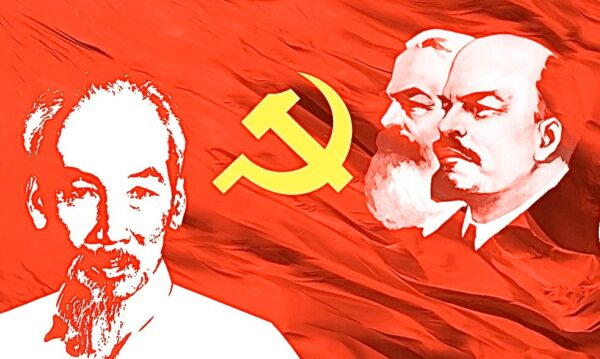
\includegraphics[scale=0.5]{images/CPV-logo}
\end{center}
\end{figure}
\vskip 3 cm
\begin{center}
\fontsize{18}{14}\selectfont
\textbf{GIÁO TRÌNH}\\
\fontsize{20}{16}\selectfont
\textbf{LỊCH SỬ ĐẢNG CỘNG SẢN VIỆT NAM}\\
\fontsize{18}{12}\selectfont
\textbf{(Sử dụng trong các trường đại học $-$ hệ không chuyên lý luận chính trị)}
\end{center}
\vskip 1 cm
\vskip 3 cm
\begin{center}
\textbf{HÀ NỘI, THÁNG 9 NĂM 2019}
\end{center}
\end{mybox}
\end{titlepage}

\begin{center}
\textbf{CHỈ ĐẠO BIÊN SOẠN}\\
Đồng chí \textbf{Võ Văn Thưởng}, Ủy viên Bộ Chính trị khóa XII,\\
Bí thư Trung ương Đảng khóa XII, Trưởng Ban Tuyên giáo Trung ương khóa XII.\\
Đồng chí GS. TS. \textbf{Phùng Xuân Nhạ}, Ủy viên Trung ương Đảng khóa XII,\\
Bộ trưởng Bộ Giáo dục và Đào tạo nhiệm kỳ 2016 $-$ 2021.\\
Đồng chí PGS. TS. \textbf{Phạm Văn Linh}, Phó Chủ tịch Hội đồng Lý luận Trung ương khóa XII,\\
Trưởng Ban Chỉ đạo biên soạn giáo trình các môn Lý luận chính trị.
\end{center}

\vskip 2 cm
\begin{center}
\textbf{HỘI ĐỒNG BIÊN SOẠN}
\end{center}

\begin{enumerate}
\item PGS. TS. Nguyễn Trọng Phúc, Chủ tịch Hội đồng.
\item PGS. TS. Ngô Đăng Trí, Phó Chủ tịch Hội đồng.
\item PSG. TS. Nguyễn Ngọc Hà, Thư ký chuyên môn.
\item Thiếu tướng, PGS. TS. Nguyễn Bình Ban, Ủy viên.
\item PGS. TS. Vũ Quang Hiển, Ủy viên.
\item PGS. TS. Phạm Xuân Mỹ, Ủy viên.
\item PGS. TS. Nguyễn Mạnh Hà, Ủy viên.
\item TS. Nguyễn Hữu Công, Ủy viên.
\item Đại tá, PGS. TS. Nguyễn Văn Sự, Ủy viên.
\item PGS. TS. Nguyễn Văn Giang, Ủy viên.
\item PGS. TS. Trần Thị Thu Hương, Ủy viên.
\item TS. Nguyễn Thị Hoàn, Ủy viên.
\item TS. Dương Văn Kha, Ủy viên.
\item TS. Ngô Quang Định, Ủy viên.
\item Nguyễn Đức Trung, Thư ký hành chính.
\end{enumerate}

\begin{center}
\textbf{\textit{(Theo quyết định số 5001/QĐ-BGDĐT, ngày 29 tháng 1 năm 2017, của Bộ trưởng Bộ Giáo dục và Đào tạo)}}
\end{center}
\newpage

\section*{Lời mở đầu}
Thực hiện kết luận số 94-KL/TW của Ban Bí thư Trung ương Đảng, ngày 28/3/2014, "Về tiếp tục đổi mới học tập lý luận chính trị trong hệ thống giáo dục quốc dân"; thực hiện Quyết định số 5001/QĐ-BGDĐT của Bộ trưởng Bộ Giáo dục và Đào tạo, ngày 29/11/2017, về việc thành lập Hội đồng biên soạn chương trình, giáo trình môn học \textit{Lịch sử Đảng Cộng sản Việt Nam} của các chuyên ngành đào tạo chuyên và không chuyên về lý luận chính trị trình độ đại học, nhiệm vụ biên soạn đã được \textit{Hội đồng biên soạn} triển khai nghiêm túc, đúng tiến độ theo định hướng của lãnh đạo Ban Tuyên giáo Trung ương, lãnh đạo Bộ Giáo dục và Đào tạo, trực tiếp là Ban Chỉ đạo.

Quá trình biên soạn giáo trình, Hội đồng đã kế thừa các giáo trình Lịch sử Đảng Cộng sản Việt Nam của Hội đồng Trung ương chỉ đạo biên soạn giáo trình quốc gia các môn lý luận Mác $-$ Lênin và tư tưởng Hồ Chí Minh, giáo trình của Bộ Giáo dục và Đào tạo và giáo trình của Học viện Chính trị quốc gia Hồ Chí Minh. Giáo trình biên soạn lần này cho cả hai hệ cố gắng thể hiện rõ những kết quả nghiên cứu mới của khoa học Lịch sử Đảng Cộng sản Việt Nam, những tổng kết và kết luận của các Đại hội Đảng toàn quốc và một số Hội nghị Trung ương, bảo đảm tính Đảng và tính khoa học. Với hệ chuyên lý luận chính trị, nội dung sâu hơn, nhất là các Cương lĩnh và những bài học lớn trong sự lãnh đạo của Đảng hướng vào làm rõ một số vấn đề có tính quy luật, lý luận của cách mạng Việt Nam.

Các Cương lĩnh của Đảng (2/1930, 10/1930, 3/1951, 6/1991 và Cương lĩnh xây dựng đất nước trong thời kỳ quá độ lên chủ nghĩa xã hội (bổ sung, phát triển năm 2011)) được trình bày gắn với các chương về các thời kỳ lịch sử. Nhiệm vụ xây dựng chủ nghĩa xã hội và bảo vệ miền Bắc (1954 $-$ 1975) được trình bày trong Chương 2 về hai cuộc kháng chiến giành độc lập hoàn toàn và thống nhất Tổ quốc.

Hội đồng biên soạn đã nhận được sự quan tâm chỉ đạo của đồng chí Võ Văn Thưởng, Ủy viên Bộ Chính trị khóa XII, Bí thư Trung ương Đảng khóa XII, Trưởng Ban Tuyên Giáo Trung ương khóa XII; GS. TS. Phùng Xuân Nhạ, Ủy viên Trung ương Đảng khóa XII, Bộ trưởng Bộ Giáo dục và Đào tạo nhiệm kỳ 2016 $-$ 2021; PGS. TS. Phạm Văn Linh, Phó Chủ tịch Hội đồng Lý luận Trung ương khóa XII, Trưởng Ban Chỉ đạo biên soạn giáo trình các môn Lý luận chính trị. 

Hội đồng biên soạn đã nhận được ý kiến đóng góp cả về nội dung và kết cấu giáo trình của các thầy, cô giáo trực tiếp giảng dạy môn Lịch sử Đảng Cộng sản Việt Nam ở các Học viện, trường đại học trong cả nước qua các cuộc hội thảo, tọa đàm, tập huấn và giảng dạy thí điểm. Hội đồng đã nhận được ý kiến đóng góp trực tiếp của các nhà khoa học: GS. TS. Phùng Hữu Phú, GS. TS. Nguyễn Ngọc Cơ, PSG. TS. Trần Đức Cường, PGS. TS. Đoàn Ngọc Hải, PGS. TS. Trịnh Đình Tùng, PGS. TS. Bùi Kim Đỉnh, PGS. TS. Nguyễn Danh Tiên, PGS. TS. Nguyễn Xuân Tú, PGS. TS. Huỳnh Thị Gấm, TS. Đào Thị Bích Hồng, PGS. TS. Nguyễn Đình Lê, TS. Nguyễn Thị Thanh Huyền, TS. Nguyễn Đình Cả và nhiều nhà khoa học khác.

Mặc dù đã có nhiều cố gắng trong biên soạn, bổ sung, song giáo trình khó tránh khỏi những thiếu sót, hạn chế. Quá trình giảng dạy, học tập rất mong được tiếp tục bổ sung, tu chỉnh để không ngừng nâng cao chất lượng giáo trình môn học Lịch sử Đảng Cộng sản Việt Nam.

\begin{flushright}
\textbf{HỘI ĐỒNG BIÊN SOẠN}
\end{flushright}
\newpage

\tableofcontents

\setcounter{page}{1}
\pagenumbering{arabic}
\chapter{Chương nhập môn: Đối tượng, chức năng, nhiệm vụ, nội dung và phương pháp nghiên cứu, học tập Lịch sử Đảng Cộng sản Việt Nam}
Đảng Cộng sản Việt Nam do Chủ tịch Hồ Chí Minh sáng lập ngày 03/2/1930. Từ thời điểm lịch sử đó, lịch sử của Đảng hòa quyện cùng lịch sử của dân tộc. Đảng đã lãnh đạo và đưa sự nghiệp cách mạng của giai cấp công nhân và dân tộc Việt Nam đi từ thắng lợi này đến thắng lợi khác, "có được cơ đồ và vị thế như ngày nay" \footfullcite[tr. 20]{HNTW4K12}. "\textit{Đảng Cộng sản Việt Nam} là đội tiền phong của giai cấp công nhân, đồng thười là đội tiền phong của nhân dân lao động và của dân tộc Việt Nam, đại biểu trung thành lợi ích của giai cấp công nhân, nhân dân lao động và của dân tộc. Đảng lấy chủ nghĩa Mác $-$ Lênin và tư tưởng Hồ Chí Minh làm nền tảng tư tưởng, kim chỉ nam cho hành động, lấy tập trung dân chủ làm nguyên tắc tổ chức cơ bản" \footfullcite[tr. 88]{DH11}.

Lịch sử Đảng Cộng sản Việt Nam là một chuyên ngành, một bộ phận của khoa học lịch sử. Chuyên ngành lịch sử Đảng Cộng sản Việt Nam đã được nghiên cứu từ rất sớm. Năm 1933, tác giả Hồng Thế Công (tức Hà Huy Tập) đã công bố tác phẩm \textit{Sơ thảo lịch sử phong trào cộng sản Đông Dương}. Ở các thời kỳ lịch sử của Đảng, Hồ Chí Minh và các nhà lãnh đạo đã trình bày lịch sử và có những tổng kết quan trọng. Đại hội đại biểu toàn quốc lần thứ III của Đảng (1960) đã nêu rõ nhiệm vụ nghiên cứu, tổng kết lịch sử Đảng, nhất là tổng kết kinh nghiệm, bài học lãnh đạo của Đảng, con đường và quy luật phát triển của cách mạng Việt Nam.

Năm 1962, cơ quan chuyên trách nghiên cứu, biên soạn lịch sử Đảng là Ban Nghiên cứu Lịch sử Đảng Trung ương được thành lập (nay là Viện Lịch sử Đảng). Từ những năm 60 của thế kỷ XX, bộ môn lịch sử Đảng đã được giảng dạy, học tập chính thức trong các trường đại học, cao đẳng, trung cấp chuyên nghiệp. Theo sự chỉ đạo của Bộ Chính trị khóa VII, ngày 13/7/1992, Chủ tịch Hội đồng Bộ trưởng (nay là Thủ tướng Chính phủ) đã ban hành Quyết định số 255CT thành lập Hội đồng chỉ đạo biên soạn giáo trình quốc gia các bộ môn khoa học Mác - Lênin, tư tưởng Hồ Chí Minh, trong đó có bộ môn Lịch sử Đảng Cộng sản Việt Nam.

Giáo trình bộ môn Lịch sử Đảng Cộng sản Việt Nam dùng trong các trường đại học được biên soạn lần này là sự kế thừa và phát triển các giáo trình đã biên soạn trước đây, phù hợp với yêu cầu đổi mới căn bản, toàn diện giáo dục và đào tạo theo quan điểm của Đảng.

\section{Đối tượng nghiên cứu của môn học Lịch sử Đảng Cộng sản Việt Nam}
\textit{Đối tượng nghiên cứu của khoa học Lịch sử Đảng là sự ra đời, phát triển và hoạt động lãnh đạo của Đảng qua các thời kỳ lịch sử.}

\begin{enumerate}
\item Trước hết là các sự kiện lịch sử Đảng. Cần phân biệt rõ sự kiện lịch sử Đảng gắn trực tiếp với sự lãnh đạo của Đảng. Phân biệt sự kiện lịch sử Đảng với sự kiện lịch sử dân tộc và lịch sử quân sự trong cùng thời kỳ, thời điểm lịch sử. Môn học lịch sử Đảng Cộng sản Việt Nam nghiên cứu sâu sắc, có hệ thống \textit{các sự kiện lịch sử Đảng}, hiểu rõ nội dung, tính chất, bản chất, của các sự kiện đó gắn liền với sự lãnh đạo của Đảng. Các sự kiện thể hiện quá trình Đảng ra đời, phát triển và lãnh đạo sự nghiệp giải phóng dân tộc, kháng chiến cứu quốc và xây dựng, phát triển đất nước theo con đường xã hội chủ nghĩa, trên các lĩnh vực chính trị, quân sự, kihn tế, xã hội, văn hóa, quốc phòng, an ninh, đối ngoại, ...

Sự kiện lịch sử Đảng là hoạt động lãnh đạo, đấu tranh phong phú và oanh liệt của Đảng làm sáng rõ bản chất cách mạng của Đảng với tư cách là một đảng chính trị, "là đội tiên phong của giai cấp công nhân, đồng thời là đội tiên phong của nhân dân lao động và của dân tộc Việt Nam, đại biểu trung thành lợi ích của giai cấp công nhân, nhân dân lao động và của dân tộc". Hệ thống các sự kiện lịch sử Đảng làm rõ thắng lợi, thành tựu của cách mạng, đồng thời cũng thấy rõ những khó khăn, thách thức, hiểu rõ những hi sinh, cống hiến lớn lao của toàn Đảng, toàn dân, toàn quân, sự hi sinh, phấn đấu của các tổ chức lãnh đạo của Đảng từ Trung ương tới cơ sở, của mỗi cán bộ, đảng viên, với những tấm gương tiêu biểu. Các sự kiện phải được tái hiện trên cơ sở tư liệu lịch sử chính xác, trung thực, khách quan.
\item Đảng lãnh đạo cách mạng giải phóng dân tộc, xây dựng và phát triển đất nước bằng \textit{Cương lĩnh, đường lối, chủ trương, chính sách lớn}. Lịch sử Đảng có đối tượng nghiên cứu là Cương lĩnh, đường lối của Đảng, phải nghiên cứu, làm sáng tỏ nội dung Cương lĩnh, đường lối của Đảng, cơ sở lý luận, thực tiễn và giá trị hiện thực của đường lối trong tiến trình phát triển của cách mạng Việt Nam. Cương lĩnh, đường lối đúng đắn là điều kiện trước hết quyết định thắng lợi của cách mạng. Phải không ngừng bổ sung, phát triển đường lối phù hợp với sự phát triển của lý luận và thực tiễn và yêu cầu của cuộc sống; chống nguy cơ sai lầm về đường lối, nếu sai lầm về đường lối sẽ dẫn tới đổ vỡ, thất bại.

Đảng đề ra Cương lĩnh chính trị đầu tiên (2/1930); Luận chương chính trị (10/1930); Chính cương của Đảng (2/1951); Cương lĩnh xây dựng đất nước trong thời kỳ quá độ lên chủ nghĩa xã hội (6/1991) và bổ sung, phát triển năm 2011. Quá trình lãnh đạo, Đảng đề ra đường lối nhằm cụ thể hóa Cương lĩnh trên những vấn đề nổi bật ở mỗi thời kỳ lịch sử. Đường lối cách mạng giải phóng dân tộc. Đường lối kháng chiến bảo vệ Tổ quốc. Đường lối cách mạng dân tộc dân chủ nhân dân. Đường lối cách mạng xã hội chủ nghĩa. Đường lối đổi mới. Đường lối quân sự. Đường lối đối ngoại v.v. Đảng quyết định những vấn đề chiến lược, sách lược và phương pháp cách mạng. Đảng là người tổ chức phong trào cách mạng của quần chúng nhân dân hiện thực hóa đường lối đưa đến thắng lợi.

\item Đảng lãnh đạo thông qua quá trình \textit{chỉ đạo, tổ chức} thực tiễn trong tiến trình cách mạng. Nghiên cứu, học tập lịch sử Đảng Cộng sản Việt Nam làm rõ \textit{thắng lợi, thành tựu, kinh nghiệm, bài học của cách mạng Việt Nam} do Đảng lãnh đạo trong sự nghiệp giải phóng dân tộc, kháng chiến giành độc lập, thống nhất, thành tựu của công cuộc đổi mới. Từ một quốc gia phong kiến, kinh tế nông nghiệp lạc hậu, một nước thuộc địa, bị đế quốc, thực dân cai trị, dân tộc Việt Nam đã giành lại độc lập bừng cuộc Cách mạng tháng Tám năm 1945 với bản \textit{Tuyên ngôn độc lập} lịch sử; tiến hành hai cuộc kháng chiến giải phóng, bảo vệ Tổ quốc, thống nhất đất nước; thực hiện công cuộc đổi mới đưa đất nước quá độ lên chủ nghĩa xã hội với những thành tựu to lớn, có ý nghĩa lịch sử. Đảng cũng thẳng thắn nêu rõ những khuyết điểm, hạn chế, khó khăn, thách thức, nguy cơ cần phải khắc phục, vượt qua.

Nghiên cứu, học tập lịch sử Đảng là giáo dục sâu sắc những kinh nghiệm, bài học trong lãnh đạo của Đảng. Tổng kết kinh nghiệm, bài học, tìm ra quy luật riêng của cách mạng Việt Nam là công việc thường xuyên của Đảng ở mỗi thời kỳ lịch sử. Đó là nội dung và yêu cầu của công tác lý luận, tư tưởng của Đảng, nâng cao trình độ lý luận, trí tuệ của Đảng. Lịch sử Đảng là quá trình nhận thức, vận dụng và phát triển sáng tạo chủ nghĩa Mác - Lênin, tư tưởng Hồ Chí Minh vào thực tiễn Việt Nam. Cần nhận thức rõ và chú trọng giáo dục những truyền thống nổi bật của Đảng; truyền thống đấu tranh kiên cường, bất khuất của Đảng; truyền thống đoàn kết, thống nhất trong Đảng; truyền thống gắn bó mật thiết với nhân dân, vì lợi ích quốc gia, dân tộc; truyền thống của chủ nghĩa quốc tế trong sáng.
\item Nghiên cứu Lịch sử Đảng là làm rõ hệ thống tổ chức Đảng, công tác xây dựng Đảng qua các thời kỳ lịch sử. Nghiên cứu, học tập lịch sử Đảng để nêu cao hiểu biết về \textit{công tác xây dựng Đảng trong các thời kỳ lịch sử} về chính trị, tư tưởng, tổ chức và đạo đức. Xây dựng Đảng về chính trị bảo đảm tính đúng đắn của đường lối, củng cố chính trị nội bộ và nâng cao bản lĩnh chính trị của Đảng. Xây dựng Đảng về tư tưởng "Đảng lấy chủ nghĩa Mác $-$ Lênin, tư tưởng Hồ Chí Minh làm nền tảng tư tưởng, kim chỉ nam cho hành động. Xây dựng Đảng về tổ chức, củng cố, phát triển hệ thống tổ chức và đội ngũ cán bộ, đảng viên của Đảng, tuân thủ các nguyên tắc tổ chức cơ bản". Xây dựng Đảng về đạo đức với những chuẩn mực về đạo đức trong Đảng và ngăn chặn, đẩy lùi sự suy thoái đạo đức, lối sống của một bộ phận cán bộ, đảng viên hiện nay.
\end{enumerate}
\section{Chức năng, nhiệm vụ của môn học Lịch sử Đảng Cộng sản Việt Nam}
Là một ngành của khoa học lịch sử, Lịch sử Đảng Cộng sản Việt Nam có chức năng, nhiệm vụ của khoa học lịch sử, đồng thời có những điểm cần nhấn mạnh.
\subsection{Chức năng của khoa học Lịch sử Đảng}
Trước hết đó là \textit{chức năng nhận thức}. Nghiên cứu và học tập lịch sử Đảng Cộng sản Việt Nam để nhận thức đầy đủ, có hệ thống những tri thức lịch sử lãnh đạo, đấu tranh và cầm quyền của Đảng, nhận thức rõ về Đảng với tư cách một Đảng chính trị $-$ tổ chức lãnh đạo của giai cấp công nhân, nhân dân lao động và dân tộc Việt Nam. Quy luật ra đời và phát triển của Đảng là sự kết hợp chủ nghĩa Mác $-$ Lênin với phong trào công nhân và phong trào yêu nước Việt Nam. Đảng được trang bị học thuyết lý luận, có Cương lĩnh, đường lối rõ ràng, có tổ chức, kỷ luật chặt chẽ, hoạt động có nguyên tắc. Từ năm 1930 đến nay, Đảng là tổ chức lãnh đạo duy nhất của cách mạng Việt Nam. TỪ Cách mạng tháng Tám năm 1945, Đảng trở thành Đảng cầm quyền, nghĩa là Đảng nắm chính quyền, lãnh đạo Nhà nước và xã hội. Sự lãnh đạo đúng đắn của Đảng là nhân tố hàng đầu quyết định thắng lợi của cách mạng. Đảng thường xuyên tự xây dựng và chỉnh đốn để hoàn thành sứ mệnh lịch sử trước đất nước và dân tộc.

Nghiên cứu, học tập lịch sử Đảng Cộng sản Việt Nam còn nhằm nâng cao nhận thức về thời đại mới của dân tộc $-$ thời đại Hồ Chí Minh, góp phần bồi đắp nhận thức lý luận từ thực tiễn Việt Nam. Nâng cao nhận thức về giác ngộ chính trị, góp phần làm rõ những vấn đề của khoa học chính trị (chính trị học) và khoa học lãnh đạo, quản lý. Nhận thức rõ những vấn đề lớn của đất nước, dân tộc trong mối quan hệ với những vấn đề của thời đại và thế giới. Tổng kết lịch sử Đảng để nhận thức quy luật của cách mạng giải phóng dân tộc, xây dựng và bảo vệ Tổ quốc, quy luật đi lên chủ nghĩa xã hội ở Việt Nam. Năng lực nhận thức và hành động theo quy luật là điều kiện bảo đảm sự lãnh đạo đúng đắn của Đảng. 

Nghiên cứu, biên soạn, giảng dạy, học tập lịch sử Đảng Cộng sản Việt Nam cần quán triệt \textit{chức năng giáo dục} của khoa học lịch sử. Giáo dục sâu sắc tinh thần yêu nước, ý thức, niềm tự hào, tự tôn, ý chí tự lực, tự cường dân tộc. Tinh thần đó hình thành trong lịch sử dụng nước, giữ nước của dân tộc và phát triển đến đỉnh cao ở thời kỳ Đảng lãnh đạo sự nghiệp cách mạng của dân tộc. Lịch sử Đảng Cộng sản Việt Nam giáo dục lý tưởng cách mạng với mục tiêu chiến lược là độc lập dân tộc và chủ nghĩa xã hội. Đó cũng là sự giáo dục tư tưởng chính trị, nâng cao nhận thức tư tưởng, lý luận, con đường phát triển của cách mạng và dân tộc Việt Nam. Lịch sử Đảng Cộng sản Việt Nam giáo dục chủ nghĩa anh hùng cách mạng, tinh thần chiến đấu bất khuất, đức hi sinh, tính tiên phong gương mẫu của các tổ chức đảng, những chiến sĩ cống sản tiêu biểu trong sự nghiệp đấu tranh giải phóng dân tộc và phát triển đất nước. Lịch sử Đảng Cộng sản Việt Nam có vai trò quan trọng trong giáo dục truyền thống của Đảng và dân tộc, góp phần giáo dục đạo đức cách mạng, nhân cách, lối sống cao đẹp như Hồ Chí Minh khẳng định: "Đảng ta là đạo đức, là văn minh".

Cùng với hai chức năng cơ bản của sử học là \textit{nhận thức} và \textit{giáo dục}, khoa học lịch sử Đảng còn có chức năng \textit{dự báo} và \textit{phê phán}. Từ nhận thức những gì đã diễn ra trong quá khứ để hiểu rõ hiện tại và dự báo tương lai của sự phát triển. Năm 1942, trong tác phẩm \textit{Lịch sử nước ta}, Hồ Chí Minh đã dự báo: "Năm 1945 Việt Nam độc lập". Sau này, Người còn nhiều lần dự báo chính xác trong 2 cuộc kháng chiến. Lãnh đạo đòi hỏi phải thấy trước. Hiện nay, Đảng nhấn mạnh năng lực tự dự báo. Để tăng cường sự lãnh đạo, nâng cao sức chiến đấu của Đảng, tự phê bình và phê bình là quy luật phát triển của Đảng. Phải kiên quyết phê phán những biểu hiện tiêu cực, lạc hậu, hư hỏng. Hiện nay, sự phê phán nhằm ngăn chặn, đẩy lùi sự suy thoái về tư tưởng chính trị, đạo đức, lối sống và những biểu hiện "tự diễn biến", "tự chuyển hóa" trong nội bộ.

\subsection{Nhiệm vụ của khoa học lịch sử Đảng}
Nhiệm vụ của khoa học lịch sử Đảng được đặt ra từ đối tượng nghiên cứu đồng thười cụ thể hóa chức năng của khoa học lịch sử Đảng.
\begin{itemize}
\item \textit{Nhiệm vụ trình bày có hệ thống Cương lĩnh, đường lối của Đảng}. Khoa học lịch sử Đảng có \textit{nhiệm vụ hằng đầu là khẳng định, chứng minh giá trị khoa học và hiện thực của những mục tiêu chiến lược và sách lược cách mạng} mà Đảng đề ra trong Cương lĩnh, đường lối từ khi Đảng ra đời và suốt quá trình lãnh đạo cách mạng. Mục tiêu và con đường đó là sự kết hợp, thống nhất giữa thực tiễn lịch sử với nền tảng lý luận nhằm thúc đẩy tiến trình cách mạng, nhận thức và cải biến đất nước, xã hội theo con đường đúng đắn. Sự lựa chọn mục tiêu độc lập dân tộc gắn liền với chủ nghĩa xã hội phù hợp với quy luật tiến hóa của lịch sử, đã và đang được hiện thực hóa.
\item \textit{Nhiệm vụ tái hiện tiến trình lịch sử lãnh đạo, đấu tranh của Đảng}. Từ hiện thực lịch sử và các nguồn tư liệu thành văn và không thành văn, \textit{khoa học lịch sử Đảng có nhiệm vụ rất quan trọng là làm rõ những sự kiện lịch sử, làm nổi bật các thời kỳ, giai đoạn và dấu mốc phát triển căn bản của tiến trình lịch sử}, nghĩa là tái hiện quá trình lịch sử lãnh đạo và đấu tranh của Đảng. Những kiến thức, tri thức lịch sử Đảng được làm sáng tỏ từ vai trò lãnh đạo, hoạt động thực tiễn của Đảng, vai trò, sức mạnh của nhân dân, của khối đại đoàn kết toàn dân tộc. Hoạt động của Đảng không biệt lập mà thống nhất và khơi dậy mạnh mẽ nguồn sức mạnh từ giai cấp công nhân, nhân dân lao động và toàn dân tộc.
\item \textit{Nhiệm vụ tổng kết lịch sử của Đảng}. Lịch sử Đảng Cộng sản Việt nam không dừng lại mô tả, tái hiện sự kiện và tiến trình lịch sử, mà còn \textit{có nhiệm vụ tổng kết từng chặng đường và suốt tiến trình lịch sử, làm rõ kinh nghiệm, bài học, quy luật và những vấn đề lý luận} của cách mạng Việt Nam. Kinh nghiệm lịch sử gắn liền với những sự kiện hoặc một giai đoạn lịch sử nhất định. Bài học lịch sử khái quát cao hơn gắn liền với một thời kỳ dài, một vấn đề của chiến lược cách mạng hoặc khái quát toàn bộ tiến trình lịch sử của Đảng. Quy luật và những vấn đề lý luận ở tầm tổng kết cao hơn. Hồ Chí Minh nêu rõ:

"Lý luận là đem \textit{thực tế} trong lịch sử, trong kinh nghiệm, trong các cuộc tranh đấu, xem xét, so sánh thật kỹ lưỡng, rõ ràng, làm thành kết luận. Rồi lại đem nó chứng minh với thực tế. Đó là lý luận chân chính" \footfullcite[tr. 273]{HCMtt5}.

"Lý luận do kinh nghiệm cách mạng ở các nước và trong nước ta, do kinh nghiệm từ trước và kinh nghiệm hiện nay gom góp phân tích và kết luận những kinh nghiệm đó thành ra lý luận" \footfullcite[tr. 312]{HCMtt5}.

Hồ Chí Minh nhiều lần đặt ra yêu cầu phải tổng kết, tìm ra quy luật riêng của cách mạng Việt Nam. Qua nhiều lần tổng kết, Đàng Cộng sản Việt Nam khẳng định:

"Con đường đi lên chủ nghĩa xã hội ở nước ta ngày càng được xác định rõ hơn" \footfullcite[tr. 356]{VKDtt55}.

"Con đường đi lên chủ nghĩa xã hội ở nước ta là phù hợp với thực tiễn của Việt Nam và xu thế phát triển của lịch sử" \footfullcite[tr. 66]{DH12}.
\item Một nhiệm vụ quan trọng của lịch sử Đảng là làm rõ vai trò, sức chiến đấu của hệ thống tổ chức đảng từ Trung ương ddeeens cơ sở trong lãnh đạo, tổ chức thực tiễn. Những truyền thống nổi bật của Đảng. Trí tuệ, tính tiên phong, gương mẫu, bản lĩnh của cán bộ, đảng viên. Tấm gương của Chủ tịch Hồ Chí Minh và các nhà lãnh đạo, những chiến sĩ cộng sản tiêu biểu trong các thời kỳ cách mạng. Những giá trị truyền thống, đức hi sinh và tấm gương tiêu biểu luôn luôn là động lực cho sự phát triển và bản chất cách mạng của Đảng. Nghị quyết Trung ương 4 khóa XII (tháng 10/2016) khẳng định: "Chúng ta có quyền tự hào về bản chất tốt đẹp, truyền thống anh hùng và lịch sử vẻ vang của Đảng ta $-$ Đảng của Chủ tịch Hồ Chí Minh vĩ đại, đại biểu của dân tộc Việt Nam anh hùng". Có một nhiệm vụ là hoàn thiện hệ thống tư liệu lịch sử Đảng.
\end{itemize}
\section{Phương pháp nghiên cứu, học tập môn học Lịch sử Đảng Cộng sản Việt Nam}
\subsection{Quán triệt phương pháp luận sử học}
Phương pháp nghiên cứu, học tập Lịch sử Đảng Cộng sản Việt Nam cần dựa trên phương pháp luận khoa học mác xít, đặc biệt là nắm vững chủ nghĩa duy vật biện chứng và chủ nghĩa duy vật lịch sử để xem xét và nhận thức lịch sử một cách khách quan, trung thực và đúng quy luật. Chú trọng nhận thức lịch sử theo quan điểm khách quan, toàn diện, phát triển và lịch sử cụ thể. Tư duy từ thực tiễn, từ hiện thực lịch sử, coi thực tiễn và kết quả của hoạt động thực tiễn là tiêu chuẩn cho chân lý. Chân lý là cụ thể, cách mạng là sáng tạo. Nhận thức rõ các sự kiện và tiến trình lịch sử trong các quan hệ: nguyên nhân và kết quả, hình thức và nội dung, hiện tượng và bản chất, cái chung và cái riêng, phổ biến và đặc thù.

Chủ nghĩa duy vật lịch sử là kết quả của tư duy biện chứng, khoa học để xem xét, nhận thức lịch sử. Khi nghiên cứu, học tập lịch sử Đảng Cộng sản Việt Nam, cần thiết phải nhận thức, vận dụng chủ nghĩa duy vật lịch sử để nhận thức tiến trình cách mạng do Đảng Cộng sản Việt Nam lãnh đạo. Lý luận về hình thái kinh tế $-$ xã hội; về giai cấp và đấu tranh giai cấp; về dân tộc và đấu tranh dân tộc; về vai trò của quần chúng nhân dân và cá nhân trong lịch sử; về cách mạng xã hội chủ nghĩa và tính tất yếu của cách mạng xã hội chủ nghĩa, sứ mệnh lịch sử của giai cấp vô sản và Đảng Cộng sản.

Cùng với chủ nghĩa Mác $-$ Lênin, tư tưởng Hồ Chí Minh là nền tảng tư tưởng và kim chỉ nam cho hành động của Đảng. Tư tưởng Hồ Chí Minh dẫn dắt sự nghiệp cách mạng của Đảng và dân tộc. Nghiên cứu, nắm vững tư tưởng Hồ Chí Minh có ý nghĩa quan trọng để hiểu rõ lịch sử Đảng. Tư tưởng Hồ Chí Minh và tư duy, phong cách khoa học của Người là cơ sở và định hướng về phương pháp nghiên cứu, học tập Lịch sử Đảng Cộng sản Việt Nam, không ngừng sáng tạo, chống chủ nghĩa giáo điều và chủ quan duy ý chí.

\subsection{Các phương pháp cụ thể}
Khoa học lịch sử và chuyên ngành khoa học Lịch sử Đảng Cộng sản Việt Nam đều sử dụng hai phương pháp cơ bản: phương pháp lịch sử và phương pháp logic, đồng thời chú trọng vận dụng các phương pháp nghiên cứu, học tập các môn khoa học xã hội khác.
\subsubsection{Phương pháp lịch sử}
"\textit{Phương pháp lịch sử} là các con đường, cách thức tìm hiểu và trình bày quá trình phát triển của các sự vật và hiện tượng nói chung, của lịch sử loài người nói riêng với đầy đủ tính cụ thể, sống động, quanh co của chúng".

"Phương pháp lịch sử là nhằm diễn lại tiến trình phát triển của lịch sử với muôn màu muôn vẻ, nhằm thể hiện cái lịch sử với tính cụ thể, hiện thực, tính sinh động của nó. Nó giúp chúng ta nắm vững được cái lịch sử để có cơ sở nắm cái logic được sâu sắc".

Phương pháp lịch sử đi sâu vào tính muôn vẻ của lịch sử để tìm ra cái đặc thù, cái cá biệt trong cái phổ biến. Các hiện tượng lịch sử thường hay tái diễn, nhưng không bao giờ hoàn toàn như cũ; phương pháp lịch sử chú ý tìm ra cái khác trước, cái không lặp để thấy những nét đặc thù của lịch sử. Phương pháp lịch sử để thấy bước quanh co, có khi thụt lùi tạm thời của quá trình lịch sử. Phương pháp lịch sử đòi hỏi nghiên cứu thấu đáo mọi chi tiết lịch sử để hiểu vai trò, tâm lý, tình cảm của quần chúng, hiểu điểm và diện, tổng thể đến cụ thể. Chú trọng về không gian, thời gian, tên đất, tên người để tái hiện lịch sử đúng như nó đã diễn ra. Phương pháp lịch sử không có nghĩa là học thuộc lòng sự kiện, diễn biến lịch sử mà phải hiểu tính chất, bản chất của sự kiện, hiện tượng, do đó không tách rời phương pháp logic.

\subsubsection{Phương pháp logic}
"\textit{Phương pháp logic} là phương pháp nghiên cứu các hiện tượng lịch sử trong hình thức tổng quát, nhằm mục đích vạch ra bản chất, quy luật, khuynh hướng chung trong sự vận động của chúng".

Phương pháp logic đi sâu tìm hiểu cái bản chất, cái lặp lại của các hiện tượng, các sự kiện, phân tích, so sánh, tổng hợp với tư duy khái quát để tìm ra bản chất các sự kiện, hiện tượng. Xác định rõ các bước phát triển tất yếu của quá trình lịch sử để tìm ra quy luật vận động khách quan của lịch sử, phương pháp logic chú trọng những sự kiện, nhân vật, giai đoạn mang tính điển hình. Cần thiết phải nắm vững logic học và rèn luyện tư duy logic, phương pháp logic có ý nghĩa quyết định đến sự nhận thức đúng đắn thế giới khách quan, hiện thực lịch sử, thấy rõ được hướng phát triển của lịch sử. Từ nắm vững quy luật khách quan mà vận dụng vào thực tiễn cách mạng, góp phần chủ động cải tạo, cải biến thế giới và lịch sử.

Chỉ có nắm vững phương pháp lịch sử và phương pháp logic mới có thể hiểu rõ bản chất, nhận thức đúng đắn, giảng dạy và học tập Lịch sử Đảng Cộng sản Việt Nam một cách có hiệu quả, với tư cách một môn khoa học. Phương pháp lịch sử và phương pháp logic có quan hệ mật thiết với nhau và đó là sự thống nhất của phương pháp biện chứng mác xít trong nghiên cứu và nhận thức lịch sử. Các phương pháp đó không tách rời mà luôn luôn gắn với nguyên tắc tính khoa học và tính đảng trong khoa học lịch sử và trong chuyên ngành Lịch sử Đảng Cộng sản Việt Nam.

\subsubsection{Các phương pháp khác}
Cùng với hai phương pháp cơ bản là phương pháp lịch sử, phương pháp logic, nghiên cứu, học tập lịch sử Đảng Cộng sản Việt Nam cần coi trọng \textit{phương pháp tổng kết thực tiễn lịch sử} gắn với nghiên cứu lý luận để làm rõ kinh nghiệm, bài học, quy luật phát triển và những vấn đề về nhận thức lý luận của cách mạng Việt Nam do Đảng lãnh đạo. Chú trọng \textit{phương pháp so sánh}, so sánh giữa các giai đoạn, thời kỳ lịch sử, so sánh các sự kiện, hiện tượng lịch sử, làm rõ các mối quan hệ, so sánh trong nước và thế giới, v. v.

Phương pháp học tập của sinh viên, hết sức coi trọng nghe giảng trên lớp để nắm vững những nội dung cơ bản từng bài giảng của giảng viên, và nội dung tổng thể của môn học. Thực hiện \textit{phương pháp làm việc nhóm}, tiến hành thảo luận, trao đổi các vấn đề do giảng viên đặt ra để hiểu rõ hơn nội dung chủ yếu của môn học. Sử dụng công nghệ thông tin trong giảng dạy và học tập. Tổ chức các cuộc làm việc tại bảo tàng lịch sử quốc gia, bảo tàng địa phương và các di tích lịch sử đặc biệt gắn với sự lãnh đạo của Đảng. Thực hiện kiểm tra, thi cử theo đúng quy chế đào tạo của Bộ Giáo dục và Đào tạo và của các trường đại học.

Nghiên cứu, giảng dạy, học tập lịch sử Đảng Cộng sản Việt Nam cần chú trọng phương pháp vận dụng lý luận vào thực tiễn. Điều đó đòi hỏi nắm vững lý luận cơ bản của chủ nghĩa Mác $-$ Lênin, bao gồm triết học, kinh tế chính trị học, chủ nghĩa xã hội khoa học, nắm vững tư tưởng Hồ Chí Minh, luôn luôn liên hệ lý luận với thực tiễn Việt Nam để nhận thức đúng đắn bản chất của mỗi hiện tượng, sự kiện của lịch sử lãnh đạo, đấu tranh của Đảng.

Tính khoa học là sự phản ánh kết quả nghiên cứu sự vật, hiện tượng, sự kiện lịch sử phải đạt đến chân lý khách quan. Tính khoa học đòi hỏi phản ánh lịch sử khách quan, trung thực với những đánh giá, kết hợp dựa trên luận cứ khoa học, tôn trọng hiện thực lịch sử. Tính khoa học yêu cầu phương pháp nghiên cứu sáng tạo, nghiêm túc và có trách nhiệm. Tính đảng cống sản trong nghiên cứu lịch sử và lịch sử Đảng là đứng trên lập trường chủ nghĩa Mác $-$ Lênin, tư tưởng Hồ Chí Minh để nhận thức lịch sử một cách khoa học, đúng đắn; là sự phản ánh đúng đắn quan điểm, đường lối của Đảng vì lợi ích của giai cấp vô sản, của nhân dân lao động và của dân tộc; là thể hiện tính chiến đấu, biểu dương cái đúng đắn, tốt đẹp, phê phán cái xấu, cái lạc hậu, hư hỏng và những nhận thức lệch lạc, sai trái, phản động của các thế lực thù địch; luôn luôn kế thừa và phát triển sáng tạo. Tính khoa học và tính đảng là thống nhất và đều hướng tới phục vụ nhiệm vụ chính trị của Đảng, của cách mạng vì lý tưởng, mục tiêu độc lập dân tộc và chủ nghĩa xã hội.

Đối với hệ đại học không chuyên về lý luận chính trị, với phân bổ 2 tín chỉ (30 tiết giảng lý thuyết), tập trung nghiên cứu các chương tương ứng với 3 thời kỳ nổi bật của lịch sử Đảng: Đảng Cộng sản Việt Nam ra đời và lãnh đạo đấu tranh giải phóng dân tộc (1930 $-$ 1945); Đảng lãnh đạo hai cuộc kháng chiến giành độc lập hoàn toàn, thống nhất đất nước và xây dựng chủ nghĩa xã hội trên miền Bắc (1945 $-$ 1975); Đảng lãnh đạo cả nước quá độ lên chủ nghĩa xã hội, bảo vệ Tổ quốc và thực hiện công cuộc đổi mới (1975 $-$ nay). Với hệ đại học chuyên lý luận chính trị (3 tín chỉ), giảng viên giargn sâu hơn các thời kỳ lịch sử đồng thời có chương về tổng thể các bài học về sự lãnh đạo của Đảng và có thể giới thiệu có hệ thống, sâu sắc các Cương lĩnh của Đảng. Sinh viên chú trọng hơn tự nghiên cứu.

Với hệ đại học không chuyền về lý luận chính trị, sinh viên cần nắm vững có hệ thống những vấn đề cơ bản của lịch sử Đảng Cộng sản Việt Nam. Hiểu rõ đặc điểm, mâu thuẫn chủ yếu của xã hội thuộc địa, phong kiến ở Việt Nam cuối thế kỷ XIX đầu thế kỷ XX. Sự phát triển tất yếu của đấu tranh giai cấp, đấu tranh dân tộc để giải phóng dân tộc, giải phóng xã hội và giải phóng con người. Các phong trào yêu nước chống thực dân Pháp xâm ucowj \textit{từ lập trường Cần vương đến lập trường tư sản, tiểu tư sản, qua khảo nghiệm lịch sử đều lần lượt thất bại}. Tình hình đất nước \textit{đen tối như không có đường ra}. Trong hoàn cảnh đó, lãnh tụ Nguyễn Ái Quốc $-$ Hồ Chí Minh đã tìm ra con đường đấu tranh đúng đắn để tự giải phóng dân tộc, xã hội, vì cuộc sống của nhân dân. Người đã truyền bá lý luận cách mạng là chủ nghĩa Mác $-$ Lênin vào phong trào công nhân và phong trào yêu nước Việt Nam và phát triển sáng tạo học thuyết lý luận đó vào thực tiễn Việt Nam; chuẩn bị những điều kiện về tư tưởng, lý luận, chính trị, tổ chức, cán bộ để thành lập Đảng Cộng sản Việt Nam. Đảng Cộng sản Việt Nam ra đời mùa Xuân năm 1930 với Cương lĩnh chính trị đúng đắn đã mở ra thời kỳ phát triển mới của cách mạng và dân tộc Việt Nam.

Từ năm 1930 đến năm 1945, Đảng và lãnh tụ Hồ Chí Minh không ngừng bổ sung, phát triển Cương lĩnh, đường lối, giương cao ngọn cờ độc lập dân tộc theo con đường xã hội chủ nghĩa, hoàn thiện đường lối giải phóng dân tộc, lãnh đạo các phong trào cách mạng rộng lớn (1930 $-$ 1931), (1936 $-$ 1939) và cao trào giải phóng dân tộc (1939 $-$ 1945) dẫn đến thắng lợi của cuộc Cách mạng tháng Tám năm 1945. Cần nắm vững tính chất, đặc điểm, ý nghĩa lịch sử của cuộc Cách mạng tháng Tám và bản \textit{Tuyên ngôn độc lập} (02/9/1945) $-$ một thời đại mới được mở ra trong lịch sử dân tộc và cách mạng Việt Nam.

Cần hiểu được hoàn cảnh lịch sử những khó khăn, thách thức của thời kỳ mới, Đảng phải có đường lối, chiến lược và sách lược thích hợp để vừa kháng chiến vừa kiến quốc, xây dựng chính quyền nhà nước và chế độ mới. Đề ra đường lối và lãnh đạo kháng chiến làm thất bại các kế hoạch chiến tranh của thực dân Pháp đưa đến chiến thắng lịch sử Điện Biên Phủ (07/5/1954) và các nước ký kết Hiệp nghị Geneve (21/7/1954). Đế quốc Mỹ thay thế thực dân Pháp, áp đặt chủ nghĩa thực dân mới ở miền Nam Việt Nam và tiến hành cuộc chiến tranh xâm lược Việt Nam từ năm 1954 đến năm 1975 với các chiến lược chiến tranh tàn bạo chống lại dân tộc Việt Nam và phong trào cách mạng giải phóng trên thế giới. Đảng đề ra đường lối, kiên trì lãnh đạo đấu tranh, vượt qua thách thức hiểm nghèo dẫn đến toàn thắng của Chiến dịch Hồ Chí Minh lịch sử giải phóng miền Nam, thống nhất đất nước (30/4/1975).

Cần nhận thức rõ quá trình Đảng lãnh đạo cách mạng xã hội chủ nghĩa ở miền Bắc, với đường lối do Đại hội III của Đảng đề ra (9/1960) và Đảng lãnh đạo đưa cả nước quá độ lên chủ nghĩa xã hội, xây dựng và bảo vệ Tổ quốc sau năm 1975. Hiểu được quá trình đổi mới tư duy lý luận, khảo nghiệm thực tiễn trong những năm 1975 $-$ 1986 để hình thành con đường đổi mới đất nước. Nắm vững đường lối đổi mới được hoạch định tại Đại hội VI (12/1986). Sự phát triển đường lối và tổ chức thực hiện hơn 30 năm qua đưa đất nước vững bước phát triển trên con đường xã hội chủ nghĩa. Lãnh đạo cách mạng dân tộc dân chủ nhân dân, các cuộc kháng chiến, cách mạng xã hội chủ nghĩa phải vượt qua nhiều nguy cơ, khó khăn, thách thức, trong đó có cả khuyết điểm, yếu kém ở mỗi thời kỳ. Đảng đã kiên cường cùng toàn dân vượt qua, quyết tâm sửa chữa khuyết điểm, thực hiện thành công sứ mệnh lịch sử lãnh đạo cách mạng Việt Nam. Nhận thức rõ hơn những truyền thống vẻ vang của Đảng.

Hiểu rõ những vấn đề xây dựng Đảng trong lịch sử để vận dung những kinh nghiệm để làm tốt công tác xây dựng, chỉnh đốn Đảng hiện nay. Chống nguy cơ sai lầm về đường lối, nguy cơ quan liêu, tham nhũng, xa rời quần chúng và những biểu hiện tiêu cực khác. Thực hiện tốt hơn Nghị quyết Trung ương 4 khóa XII (30/10/2016) \textit{Về tăng cường xây dựng, chỉnh đốn Đảng; ngăn chặn, đẩy lùi sự suy thoái về tư tưởng chính trị, đạo đức, lối sống, những biểu hiện "tự diễn biến", "tự chuyển hóa" trong nội bộ}.

Lịch sử Đảng Cộng sản Việt Nam, như Chủ tịch Hồ Chí Minh khẳng định, \textit{là cả một pho lịch sử bằng vàng}. Đó chính là tính khoa học, giá trị thực tiễn sâu sắc trong Cương lĩnh, đường lối của Đảng; là sự lãnh đạo đúng đắn, đáp ứng kịp thời những yêu cầu, nhiệm vụ do lịch sử đặt ra; những kinh nghiệm, bài học quý báu có tính quy luật, lý luận của cách mạng Việt Nam và những truyền thống vẻ vang của Đảng. Nghiên cứu, học tập lịch sử Đảng không chỉ nắm vững những sự kiện, cột mốc lịch sử mà cần thấu hiểu những vấn đề phong phú đó trong quá trình lãnh đạo và đấu tranh, để vận dụng, phát triển trong thời kỳ đổi mới toàn diện, đẩy mạnh công nghiệp hóa, hiện đại hóa đất nước và hội nhập quốc tế.

Mục tiêu của nghiên cứu, học tập môn học lịch sử Đảng Cộng sản Việt Nam là nâng cao nhận thức, hiểu biết về Đảng Cộng sản Việt Nam $-$ đội tiền phong lãnh đạo cách mạng Việt Nam đưa đến những thắng lợi, thành tựu có ý nghĩa lịch sử to lớn trong sự phát triển của lịch sử dân tộc. Qua học tập, nghiên cứu lịch sử Đảng để giáo dục lý tưởng, truyền thống đấu tranh cách mạng của Đảng và dân tộc, củng cố, bồi đắp niềm tin đối với sự lãnh đạo của Đảng, tự hào về Đảng và thế hệ trẻ gia nhập Đảng, tham gia xây dựng Đảng ngày càng vững mạnh, tiếp tục thực hiện sứ mệnh vẻ vang của Đảng lãnh đạo bảo vệ vững chắc Tổ quốc và xây dựng thành công chủ nghĩa xã hội ở Việt Nam.

\printbibliography
\end{document}